Transfer learning is a method to consume network weights from previously trained model and applying the model 
weights in training of new convolutional neural network. The objective of the experiment was to consume the 
weights obtained from training of model with segmented data and use it in the processing of training same model 
architecture using normal pigmented skin lesions. 
\begin{figure}[!htp]
    \centering
    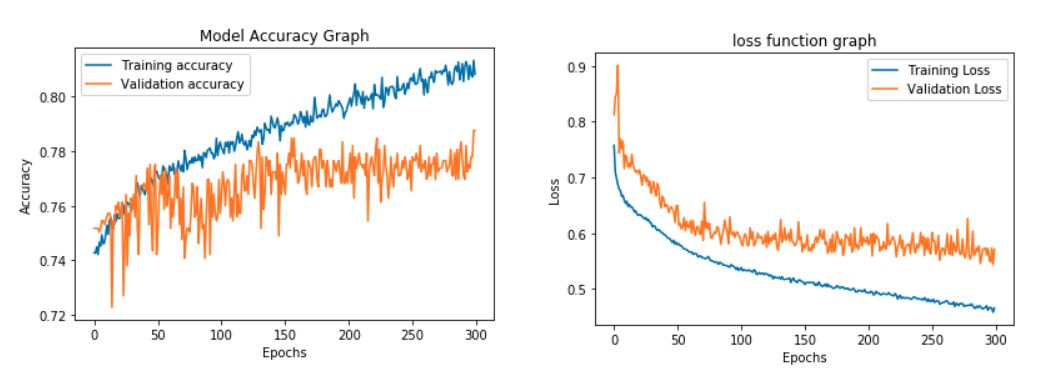
\includegraphics[width=\textwidth]{Images/transferLearning.png}
    \caption{Transfer Learning Model}
    \label{fig:translearning}
\end{figure}

The figure \ref{fig:translearning} shows the graph indicating increasing in the model accuracy for training 
and validation data and decline in the loss functoin of the model. The model was trained using the SGD optimiser 
for 300 epochs and had produced the accuracy of 79.02\% on the evaluation data. The result of applying the 
transfer learning can be observed as without applying the weights from segmented model training the accuracy 
was evaluated to be 77.4\%. Further experiments are performed using the transfer learning to evaluate the 
impact on model performance.